\documentclass{article}

% General physics constructs
\newcommand{\bra}[1]{\langle #1 |}
\newcommand{\ket}[1]{| #1 \rangle }
\newcommand{\braket}[2]{\langle #1|#2\rangle}
\newcommand{\bbraket}[3]{ \langle #1 | #2 | #3 \rangle }
\newcommand{\norm}[1]{\| #1\|}
\newcommand{\avg}[1]{\left \langle #1 \right \rangle}
\newcommand{\angavg}[1]{\left \langle #1 \right \rangle}
\newcommand{\abs}[1]{\left \lvert #1 \right \rvert}
\newcommand{\VS}{\textit{\textbf{V}}}
\newcommand{\Tr}{\textrm{Tr}}
\renewcommand{\Re}{\textrm{Re}}
\renewcommand{\Im}{\textrm{Im}}
\newcommand{\basis}[1]{\{\ket{#1}\}}

\newcommand{\omegaqubit}{\omega_{10}}

% Figures. Example usage:
% \quickfig{\columnwidth}{my_image}{This is the caption}{fig:my_fig}
\DeclareRobustCommand{\quickfig}[4]{
\begin{figure}
\begin{centering}
\includegraphics[width=#1]{#2}
\par\end{centering}
\caption{#3}
\label{#4}
\end{figure}
}

\DeclareRobustCommand{\quickwidefig}[4]{
\begin{figure*}[h]
\begin{centering}
\includegraphics[width=#1]{#2}
\par\end{centering}
\caption{#3}
\label{#4}
\end{figure*}
}

%Packages
\usepackage{amsmath}
\usepackage{amstext}
\usepackage{amssymb}
\usepackage{appendix}
\usepackage{coseoul}
\usepackage{enumerate}
\usepackage{graphicx}
\usepackage{import}
\usepackage{lscape}
\usepackage{modular}

\usepackage[pdfpagemode=UseNone,pdfstartview=FitH,colorlinks=true,linkcolor=blue,citecolor=blue,urlcolor=blue]{hyperref}
\usepackage[all]{hypcap}



\begin{document}

\section*{Tinkham Chapter 3 notes}


\subsection*{Cooper Pair Wavefunction}


\subsubsection*{Introduction}

The initial discussion in Tinkham on the BCS wavefunction relies on
equation 3.2,\begin{equation}
E-2\epsilon_{k}=\sum_{k'}V_{kk'}g_{k'}\label{eq:schrodinger}\end{equation}
which is used to show that adding a bound Cooper pair to the Fermi
vacuum actually lowers the energy of the system in certain approximations.
The discussion leading from (\ref{eq:schrodinger}) to the conclusions
that the energy is lowered is fairly clear, but it's not obvious where
(\ref{eq:schrodinger}) itself comes from. Tinkham claims that if
you stuff the wavefunction\begin{equation}
\sum_{k>k_{F}}g_{k}\cos\left(\vec{k}\cdot(\vec{x}_{1}-\vec{x}_{2})\right)\left[\alpha_{1}\beta_{2}-\beta_{1}\alpha_{2}\right]\label{eq:wavefunction_1st}\end{equation}
into the Schrodinger equation $H|\Psi\rangle=E|\Psi\rangle$, using
the Hamiltonian\begin{equation}
H=\sum_{i}\frac{p_{i}^{2}}{2m}+\frac{1}{2}\sum_{i,j}V(x_{i},x_{j})\label{eq:hamiltonian_1st}\end{equation}
you get (\ref{eq:schrodinger}). I find this difficult to understand.
It's much easier to understand what's going on if we use second quatization
so we're going to take this opportunity to demonstrate how to do things
in that formalism.


\subsubsection*{Second quantization}

The Hamiltonian for a bunch of electrons, like any charged particles,
is (ignoring spin effects) given in {}``first quantization'' by
(\ref{eq:hamiltonian_1st}) where $V(x_{i},x_{j})$ is the interaction
energy of two particles, one at $x_{i}$and the other at $x_{j}$.
Now, there's already a major problem with this Hamiltonian: the letters
$i$ and $j$ label individual particles, but we're dealing with a
system of indistinguishable particles! The very notion of counting
up the energy by summing the energies of the various particles is
silly because the notion of identity for each particle is meaningless.
Textbooks frequently teach us to deal with this problem by keeping
the form of the Hamiltonian in (\ref{eq:hamiltonian_1st}) and using
appropriately symmetrized or antisymmetrized wavefunctions. These
wavefunctions, things like $|\psi_{1}\phi_{2}\rangle+|\phi_{1}\psi_{2}\rangle$,
suffer the same problem as the Hamiltonian in that they refer to the
various particles as individual entities with labels $1$ and $2$.
The whole thing becomes a giant mess if you have lots of particles
because you have to write things in terms of determinants, and if
you have a superposition of states with different numbers of particles
it's not even clear how to write anything down at all.

This is really pretty stupid; when you use symmetrized and antisymmetrized
wavefunctions you're essentially saying to yourself {}``my notation
is not appropriate for this problem because it contains more information
than is present in the physical system, and rather than fix this fundamental
problem I'm going to add terms to my functions so as to reduce their
total information content in just the right way.'' A much more reasonable
thing to do is to realize that particles are really just excitations
of something (a {}``quantum field'' if you want) and therefore the
right way to describe a physical state is to just list the amount
of excitation in each possible field mode. For example, instead of
$|\psi_{1}\phi_{2}\rangle+|\phi_{1}\psi_{2}\rangle$ you could write
$|\psi:1,\phi:1\rangle$ meaning {}``one particle in state $\psi$
and one particle in state $\phi$.'' If you make the convention that
the states come in the order $\psi,\phi$ you could just write $|11\rangle$
instead. For a state with a superposition of total particle number
you could write something like $|10\rangle+|11\rangle$ and the meaning
is completely clear.

You can now write $\textbf{states}$ in terms of the vacuum state
by using creation/annihilation operators. For example, the state $|11\rangle$
we just discussed would be written as $|11\rangle=a_{\psi}^{\dagger}a_{\phi}^{\dagger}|0\rangle$.
Note how much simpler this is. Where before we had both particle and
state labels now we only have state labels. This makes sense since
the particles were indistinguishable in the first place we shouldn't
be labelling them at all. In fact, the notion of a particle changes
when you really understand what indistinguishability really means,
but that's a discussion for another day.

The only complication in this new language is that the creation/annihilation
operators don't always commute so you have to be careful. It turns
out that the commutation relations that make sense are\[
\left[a_{x},a_{y}^{\dagger}\right]=\delta_{xy}\qquad\textrm{Bosons (commutator) }\]
and\[
\left\{ a_{x},a_{y}^{\dagger}\right\} =\delta_{xy}\qquad\textrm{Fermions (anticommutator)}\]


Now we have to explain how to write down $\textbf{operators}$ in
this new language. Consider a generic one-body operator in the usual
quantum language\begin{eqnarray*}
\hat{O} & = & \sum_{\alpha,\beta}|\beta\rangle\langle\beta|\hat{O}|\alpha\rangle\langle\alpha|\\
\hat{O} & = & \sum_{\alpha,\beta}O_{\beta,\alpha}|\beta\rangle\langle\alpha|\end{eqnarray*}
where $O_{\beta,\alpha}$ are the matrix elements of $\hat{O}$, ie.
$O_{\beta,\alpha}\equiv\langle\beta|\hat{O}|\alpha\rangle$. What
does this operator $\emph{do}$? Whenever it finds a particle in state
$|\alpha\rangle$, it changes that particle's state to $|\beta\rangle$
and multiplies everything by the matrix element $O_{\beta,\alpha}$.
It's not hard to believe then that in the new language this would
be\[
\hat{O}=\sum_{\alpha,\beta}O_{\beta,\alpha}a_{\beta}^{\dagger}a_{\alpha}\]
because this operator does the same thing: it takes a particle from
state $|\alpha\rangle$ and puts it into $|\beta\rangle$ and multplies
everything by a matrix element. Similarly, for a two-body operator
where the matrix elements are given by $O_{\gamma,\delta,\alpha,\beta}=\langle\gamma\delta|\hat{O}|\alpha\beta\rangle$
the new version is\[
\hat{O}=\frac{1}{2}\sum_{\alpha,\beta,\gamma,\delta}O_{\gamma,\delta,\alpha,\beta}a_{\gamma}^{\dagger}a_{\delta}^{\dagger}a_{\beta}a_{\alpha}\]



\subsubsection*{Hamiltonian and Cooper pair wavefunction in second quantization}

Now we have to write down our Hamiltonian and wavefunction in second
quantization. We do the Hamiltonian first.

The Hamiltonian has kinetic and interaction terms. The matrix elements
of the kinetic energy are\[
T_{k,k'}=\delta_{k,k'}\frac{\left(\hbar k\right)^{2}}{2m}\equiv\delta_{k,k'}\epsilon_{k}\]
Therefore in second quantization we get\[
T=\sum_{k,k'}\delta_{k,k'}\epsilon_{k}a_{k}^{\dagger}a_{k'}=\sum_{k}\epsilon_{k}a_{k}^{\dagger}a_{k}=\sum_{k}\epsilon_{k}n_{k}\]
In English this says {}``The total energy is the sum over all modes
of the energy of that mode times the number of particles in that mode.''
The matrix elements of the interaction operator are\[
\langle uv|\hat{V}|xy\rangle=\delta(x-u)\delta(y-v)V(x,y)\]
Therefore, the second quantized form is\begin{eqnarray*}
\hat{V} & = & \frac{1}{2}\int_{x}\int_{y}\int_{u}\int_{v}V(x,y)\delta(x-u)\delta(y-v)a_{u}^{\dagger}a_{v}^{\dagger}a_{y}a_{x}dxdydudv\\
\hat{V} & = & \frac{1}{2}\int_{x}\int_{y}V(x,y)a_{x}^{\dagger}a_{y}^{\dagger}a_{y}a_{x}dxdy\end{eqnarray*}
To put this in the plane wave basis we Fourier Transform $a_{x}=\sum_{k}a_{k}e^{ikx}$.
Plugging this into $\hat{V}$ gives\begin{eqnarray*}
\hat{V} & = & \frac{1}{2}\sum_{k,k',p,p'}\int_{x}\int_{y}V(x,y)a_{k}^{\dagger}e^{-ik'x}a_{p}^{\dagger}e^{-ip'y}a_{p'}e^{ipy}a_{k'}e^{ikx}dxdy\\
\hat{V} & = & \frac{1}{2}\sum_{k,k',p,p'}a_{k}^{\dagger}a_{p}^{\dagger}a_{p'}a_{k'}\int_{x}\int_{y}V(x,y)e^{i(k-k')x}e^{i(p-p')y}dxdy\end{eqnarray*}
This integral is actually a bit tricky. In most physically relevant
cases the scattering potential depends only on the distance between
the particles, so $V(x,y)$ will be a function only of the difference
$x-y$. Therefore we can write the integral as\begin{eqnarray*}
\textrm{integral} & = & \int_{x}\int_{y}V(x-y)e^{i(k-k')x}e^{i(p-p')y}dxdy\\
 & = & \int_{y}e^{i(p-p')y}\int_{x}V(x-y)e^{i(k-k')x}dxdy\qquad\textrm{let }z=x-y\\
 & = & \int_{y}e^{i(p-p')y}e^{i(k-k')y}dy\int_{z}V(z)e^{i(k-k')z}dz\\
 & = & \tilde{V}(k-k')\int_{y}e^{i(p'-p+k'-k)y}dy\\
 & = & \tilde{V}(\xi)\delta(p'=p-\xi)\end{eqnarray*}
where $\xi\equiv k-k'$. Stuffing this result for the integral into
the original expression for the interaction energy gives\begin{eqnarray*}
\hat{V} & = & \frac{1}{2}\sum_{k,k',p,p'}a_{k'}^{\dagger}a_{p'}^{\dagger}a_{p}a_{k}\tilde{V}(\xi)\delta(p'=p-\xi)\\
\hat{V} & = & \frac{1----}{2}\sum_{k',k,p}a_{k'}^{\dagger}a_{p-\xi}^{\dagger}a_{p}a_{k}\tilde{V}(\xi)\\
\hat{V} & = & \frac{1}{2}\sum_{k,p,\xi}a_{k+\xi}^{\dagger}a_{p-\xi}^{\dagger}a_{p}a_{k}\tilde{V}(\xi)\end{eqnarray*}
What does this mean? The interaction Hamiltonian takes particles
from intitial momentum states $k$ and $p$ and puts them into states
$k+\xi$ and $p-\xi$ with a multiplicative factor coming from the
Fourier transform of the interaction potential at $\xi$. Basically
what this means is that the interaction can transfer a scattering
momentum $\xi$ from one particle to another. You can think of this
in terms of the so called {}``Feynman diagrams'' as shown in Figure
\ref{Flo:scattering}.

Adding the kinetic energy and scattering terms, and now including
appropriate sums over spin we get the Hamiltonian\[
H=\sum_{k,\alpha}\epsilon_{k}n_{k,\alpha}+\frac{1}{2}\sum_{k,p,\xi,\alpha,\beta}a_{k+\xi,\alpha}^{\dagger}a_{p-\xi,\beta}^{\dagger}a_{p,\beta}a_{k,\alpha}\tilde{V}(\xi)\]


%
\begin{figure}

\begin{centering}
\includegraphics[scale=0.5]{Scattering.pdf}
\par\end{centering}

\caption{The scattering of two particles through exchange of a force carrier
with momentum $\xi$.}
\label{Flo:scattering}
\end{figure}


Now let's do the wavefunction. Tinkham writes down the wavefunction
in first quantizataion in 3.1. The wavefunction we want to represent
is a filled Fermi sea plus two particles in a state with 2-body wavefunction
given by\[
\Psi(x,y)=\sum_{k}g_{k}\cos\left(\vec{k}\cdot(\vec{x}-\vec{y})\right)\left(\alpha_{x}\beta_{y}-\beta_{x}\alpha_{y}\right)\]
where here $\alpha$ and $\beta$ are the spin states and $x$ and
$y$ refer to the two particles. This wavefunction was chosen so that
the two particles make up a zero momentum state, and have a symmetric
spatial dependence so that their overlap is maximized. This maximization
of spatial overlap was chosen to anticipate the attractive interaction
between electrons.

\begin{flushleft}
In second quantization we have\[
a_{\phi,\alpha}^{\dagger}a_{\psi,\beta}^{\dagger}|0\rangle\rightarrow\phi(r_{1})\psi(r_{2})\alpha_{1}\beta_{2}-\psi(r_{1})\phi(r_{2})\beta_{1}\alpha_{2}\]
 We can use this relation to turn our 2-body wavefunction into its
second quantized form. First we separate the $x$ and $y$ dependencies\begin{eqnarray*}
\cos\left(k\cdot(x-y)\right)\left(\alpha_{1}\beta_{2}-\beta_{1}\alpha_{2}\right) & = & \frac{1}{2}\left[e^{ik\cdot x}e^{-ik\cdot y}+e^{-ik\cdot x}e^{-k\cdot y}\right]\left(\alpha_{1}\beta_{2}-\beta_{1}\alpha_{2}\right)\end{eqnarray*}
 For notational convenience rename $e^{ikx}=\phi(x)$ and $e^{-ikx}=\psi(x)$.
Then we have\begin{eqnarray*}
\cos\left(k\cdot(x-y)\right)\left(\alpha_{1}\beta_{2}-\beta_{1}\alpha_{2}\right) & = & \frac{1}{2}\left[\phi(x)\psi(y)+\psi(x)\phi(y)\right]\left(\alpha_{1}\beta_{2}-\beta_{1}\alpha_{2}\right)\\
 & = & \frac{1}{2}\left[\left(\phi(x)\psi(y)\alpha_{x}\beta_{y}-\psi(x)\phi(y)\beta_{x}\alpha_{y}\right)+\left(\psi(x)\phi(y)\alpha_{x}\beta_{y}-\phi(x)\psi(y)\beta_{x}\alpha_{y}\right)\right]\\
 & \rightarrow & \frac{1}{2}\left[a_{\phi,\alpha}^{\dagger}a_{\psi,\beta}^{\dagger}+a_{\psi,\alpha}^{\dagger}a_{\phi,\beta}^{\dagger}\right]|0\rangle\\
 & = & \frac{1}{2}\left[a_{k,\alpha}^{\dagger}a_{-k,\beta}^{\dagger}+a_{-k,\alpha}^{\dagger}a_{k,\beta}^{\dagger}\right]\end{eqnarray*}
 Notice that these terms are equal if the sign of $k$ is reversed.
Now we stuff this formula into the wavefunction,\begin{eqnarray*}
\Psi(x,y) & = & \sum_{k>k_{F}}g_{k}\cos\left(k\cdot(x-y)\right)\left(\alpha_{x}\beta_{y}-\beta_{x}\alpha_{y}\right)\\
 & \rightarrow & \sum_{k>k_{F}}g_{k}\frac{1}{2}\left[a_{k,\alpha}^{\dagger}a_{-k,\beta}^{\dagger}+a_{-k,\alpha}^{\dagger}a_{k,\beta}^{\dagger}\right]\end{eqnarray*}
This almost exactly matches Tinkham's form in 3.11 but we have an
extra term and a factor of $1/2$. It turns out that these cancel
each other as we know show. Let $\sum_{k_{F}^{+}}$ indicate a sum
over half of $k$-space, ie. the half with $k_{x}>0$. Then\[
\sum_{k>k_{F}}=\sum_{k^{+}>k_{F}}+\sum_{k^{-}>k_{F}}\]
 So\begin{eqnarray*}
\sum_{k>k_{F}}g_{k}\frac{1}{2}\left[a_{k,\alpha}^{\dagger}a_{-k,\beta}^{\dagger}+a_{-k,\alpha}^{\dagger}a_{k,\beta}^{\dagger}\right] & = & \sum_{k^{+}>k_{F}}g_{k}\frac{1}{2}\left[a_{k,\alpha}^{\dagger}a_{-k,\beta}^{\dagger}+a_{-k,\alpha}^{\dagger}a_{k,\beta}^{\dagger}\right]+\sum_{k^{-}>k_{F}}g_{k}\frac{1}{2}\left[a_{k,\alpha}^{\dagger}a_{-k,\beta}^{\dagger}+a_{-k,\alpha}^{\dagger}a_{k,\beta}^{\dagger}\right]\\
 & = & \sum_{k^{+}>k_{F}}g_{k}\frac{1}{2}a_{k,\alpha}^{\dagger}a_{-k,\beta}^{\dagger}+\sum_{k^{+}>k_{F}}g_{k}\frac{1}{2}a_{-k,\alpha}^{\dagger}a_{k,\beta}^{\dagger}+\cdots\\
 &  & \qquad\cdots+\sum_{k^{-}>k_{F}}g_{k}\frac{1}{2}a_{k,\alpha}^{\dagger}a_{-k,\beta}^{\dagger}+\sum_{k^{-}>k_{F}}g_{k}\frac{1}{2}a_{-k,\alpha}^{\dagger}a_{k,\beta}^{\dagger}\\
 & = & \sum_{k^{+}>k_{F}}g_{k}\frac{1}{2}a_{k,\alpha}^{\dagger}a_{-k,\beta}^{\dagger}+\sum_{k^{+}>k_{F}}g_{k}\frac{1}{2}a_{-k,\alpha}^{\dagger}a_{k,\beta}^{\dagger}+\cdots\\
 &  & \cdots+\sum_{k^{+}>k_{F}}g_{-k}\frac{1}{2}a_{-k,\alpha}^{\dagger}a_{k,\beta}^{\dagger}+\sum_{k^{+}>k_{F}}g_{-k}\frac{1}{2}a_{k,\alpha}^{\dagger}a_{-k,\beta}^{\dagger}\end{eqnarray*}
 Then, using the fact that $g_{k}=g_{-k}$ we have\begin{eqnarray*}
\sum_{k>k_{F}}g_{k}\frac{1}{2}\left[a_{k,\alpha}^{\dagger}a_{-k,\beta}^{\dagger}+a_{-k,\alpha}^{\dagger}a_{k,\beta}^{\dagger}\right] & = & \sum_{k^{+}>k_{F}}g_{k}a_{k,\alpha}^{\dagger}a_{-k,\beta}^{\dagger}+\sum_{k^{+}>k_{F}}g_{k}a_{-k,\alpha}^{\dagger}a_{k,\beta}^{\dagger}\\
 & = & \sum_{k>k_{F}}g_{k}a_{k,\alpha}^{\dagger}a_{-k,\beta}^{\dagger}\end{eqnarray*}
 which agrees with 3.11.
\par\end{flushleft}


\subsubsection*{Schrodinger's equation with the cooper pair wavefunction}

We now have our Cooper pair wavefunction and our Hamiltonian in second
quantized form\begin{eqnarray*}
H & = & \underbrace{\sum_{k,\alpha}\epsilon_{k}n_{k,\alpha}}_{T}+\underbrace{\frac{1}{2}\sum_{k,p,\xi,\alpha,\beta}a_{k+\xi,\alpha}^{\dagger}a_{p-\xi,\beta}^{\dagger}a_{p,\beta}a_{k,\alpha}\tilde{V}(\xi)}_{V}\\
|\Psi\rangle & = & \sum_{k>k_{F}}g_{k}a_{k,\alpha}^{\dagger}a_{-k,\beta}^{\dagger}|0\rangle\equiv\sum_{k>k_{F}}g_{k}|\psi_{k}\rangle\end{eqnarray*}
All we have to do now is plug this into the Schrodinger equation and
see what happens.\begin{eqnarray*}
H|\Psi\rangle & = & E|\Psi\rangle\\
T|\Psi\rangle+V|\Psi\rangle & = & E|\Psi\rangle\end{eqnarray*}
We work these out one term at a time.\begin{eqnarray*}
T|\Psi\rangle & = & \sum_{k',\alpha}\epsilon_{k'}n_{k',\alpha}\sum_{k>k_{F}}g_{k}|\psi_{k}\rangle\\
T|\Psi\rangle & = & \sum_{k>k_{F}}\sum_{k',\alpha}g_{k}\epsilon_{k'}n_{k',\alpha}|\psi_{k}\rangle\\
T|\Psi\rangle & = & \sum_{k>k_{F}}\sum_{k'}g_{k}\epsilon_{k'}\left(\delta_{k,k'}+\delta_{k,-k'}\right)|\psi_{k}\rangle\\
T|\Psi\rangle & = & \sum_{k>k_{F}}\left(g_{k}\epsilon_{k}+g_{-k}\epsilon_{-k}\right)|\psi_{k}\rangle\\
T|\Psi\rangle & = & 2\sum_{k>k_{F}}g_{k}\epsilon_{k}|\psi_{k}\rangle\end{eqnarray*}
where the last line is true because $g_{k}$ and $\epsilon_{k}$ are
invariant if $k$ changes sign.

Now we work out the scattering term.\begin{eqnarray*}
V|\Psi\rangle & = & \frac{1}{2}\sum_{k,p,\xi,\alpha,\beta}a_{k+\xi,\alpha}^{\dagger}a_{p-\xi,\beta}^{\dagger}a_{p,\beta}a_{k,\alpha}\tilde{V}(\xi)\sum_{k'>k_{F}}g_{k'}|\psi_{k'}\rangle\\
V|\Psi\rangle & = & \frac{1}{2}\sum_{k,p,\xi,\alpha,\beta}\sum_{k'>k_{F}}\tilde{V}(\xi)g_{k'}a_{k+\xi,\alpha}^{\dagger}a_{p-\xi,\beta}^{\dagger}a_{p,\beta}a_{k,\alpha}|\psi_{k'}\rangle\\
V|\Psi\rangle & = & \frac{1}{2}\sum_{k,p,\xi,\alpha,\beta}\sum_{k'>k_{F}}\tilde{V}(\xi)g_{k'}a_{k+\xi,\alpha}^{\dagger}a_{p-\xi,\beta}^{\dagger}\left(a_{p,\beta}a_{k,\alpha}a_{k',\sigma}^{\dagger}a_{-k',\tau}^{\dagger}\right)|0\rangle\end{eqnarray*}
The part in parentheses will be zero unless several conditions are
met. Either $p=k',\beta=\sigma$ and $k=-k',\alpha=\tau$ or vice
versa. In either case $p=-k$, so we can eliminate $p$,\[
V|\Psi\rangle=\frac{1}{2}\sum_{k,\xi,\alpha,\beta}\sum_{k'>k_{F}}\tilde{V}(\xi)g_{k'}a_{k+\xi,\alpha}^{\dagger}a_{-k-\xi,\beta}^{\dagger}\left(a_{-k,\beta}a_{k,\alpha}a_{k',\sigma}^{\dagger}a_{-k',\tau}^{\dagger}\right)|0\rangle\]
Now the term in parentheses is nonzero only when $k=k'$ or $k=-k'$.
In either case, the only spin combination of $\alpha,\beta$ that
survives is the one that matches $\sigma,\tau$, so we can reduce
everything to this\begin{eqnarray*}
V|\Psi\rangle & = & \frac{1}{2}\sum_{\xi}\sum_{k'>k_{F}}\tilde{V}(\xi)g_{k'}\left[a_{k'+\xi,\sigma}^{\dagger}a_{-k'-\xi,\tau}^{\dagger}\left(a_{-k',\tau}a_{k',\sigma}a_{k',\sigma}^{\dagger}a_{-k',\tau}^{\dagger}\right)+a_{-k'+\xi,\tau}^{\dagger}a_{k'-\xi,\sigma}^{\dagger}\left(a_{k',\sigma}a_{-k',\tau}a_{k',\sigma}^{\dagger}a_{-k',\tau}^{\dagger}\right)\right]|0\rangle\\
V|\Psi\rangle & = & \frac{1}{2}\sum_{\xi}\sum_{k'>k_{F}}\tilde{V}(\xi)g_{k'}\left[a_{k'+\xi,\sigma}^{\dagger}a_{-k'-\xi,\tau}^{\dagger}+a_{-k'+\xi,\tau}^{\dagger}a_{k'-\xi,\sigma}^{\dagger}\right]|0\rangle\\
V|\Psi\rangle & = & \frac{1}{2}\sum_{\xi}\sum_{k'>k_{F}}\tilde{V}(\xi)g_{k'}2|\psi_{k'+\xi}\rangle\\
V|\Psi\rangle & = & \sum_{\xi}\sum_{k'>k_{F}}\tilde{V}(\xi)g_{k'}|\psi_{k'+\xi}\rangle\end{eqnarray*}
Plug these forms in the Schrodinger equation to get\begin{eqnarray*}
2\sum_{k>k_{F}}g_{k}\epsilon_{k}|\psi_{k}\rangle+\sum_{k'>k_{F}}\sum_{\xi}\tilde{V}(\xi)g_{k'}|\psi_{k'+\xi}\rangle & = & E\sum_{k>k_{F}}g_{k}|\psi_{k}\rangle\\
2g_{k}\epsilon_{k}+\sum_{k'>k_{F}}\tilde{V}(k-k')g_{k'} & = & Eg_{k}\\
\left[E-2\epsilon_{k}\right]g_{k} & = & \sum_{k'>k_{F}}\tilde{V}(k-k')g_{k'}\end{eqnarray*}
This matches Tinkham's equation 3.2! I realize that this was an insanely
long discussion to get to this point, but the computation itself was
actually pretty short. If you are comfortable with second quantization
then doing the computation this way is easier than doing it with the
first quantization form of the wavefunction. This is mostly because
you don't have to write integrals and you don't have to keep track
of particle labels. If you do a computation with more than two particles
then second quantization becomes way better.


\section*{BCS ground state }

The BCS ground state is\begin{eqnarray*}
|\Psi_{G}\rangle & = & \prod_{k}(u_{k}+v_{k}c_{k\uparrow}^{\dagger}c_{-k\downarrow}^{\dagger})|0\rangle\\
\langle\Psi_{G}| & = & \langle0|\prod_{k}(u_{k}^{*}+v_{k}^{*}c_{-k\downarrow}c_{k\uparrow})\end{eqnarray*}
Here we show, as an example, how to compute the mean particle number.
We include all steps to show how to work with product states.

We would like to calculate $\bar{N}$:
\begin{align*}
\bar{N} & = \langle\Psi_{G}|\hat{N}|\Psi_{G}\rangle=\sum_{k,\sigma}\langle\Psi_{G}|\hat{n}_{k,\sigma}|\Psi_{G}\rangle \\
& = \sum_{k,\sigma}\langle0|\prod_{p}(u_{p}^{*}+v_{p}^{*}c_{-p\downarrow}c_{p\uparrow})|n_{k,\sigma}|\prod_{q}(u_{q}+v_{q}c_{q\uparrow}^{\dagger}c_{-q\downarrow}^{\dagger})|0\rangle \\
& = \sum_{k,\sigma}\langle0|(u_{k}^{*}+v_{k}^{*}c_{-k\downarrow}c_{k\uparrow})\prod_{p\neq k}(u_{p}^{*}+v_{p}^{*}c_{-p\downarrow}c_{p\uparrow})|n_{k,\sigma}|(u_{k}+v_{k}c_{k\uparrow}^{\dagger}c_{-k\downarrow}^{\dagger})\prod_{q\neq k}(u_{q}+v_{q}c_{q\uparrow}^{\dagger}c_{-q\downarrow}^{\dagger})|0\rangle \\
& = \sum_{k,\sigma}\langle0|(u_{k}^{*}+v_{k}^{*}c_{-k\downarrow}c_{k\uparrow})n_{k,\sigma}(u_{k}+v_{k}c_{k\uparrow}^{\dagger}c_{-k\downarrow}^{\dagger})\times\prod_{{q\neq k \brace p\neq k}}(u_{p}^{*}+v_{p}^{*}c_{-p\downarrow}c_{p\uparrow})(u_{q}+v_{q}c_{q\uparrow}^{\dagger}c_{-q\downarrow}^{\dagger})|0\rangle
\end{align*}
 The two terms in parentheses in the product always commute because
they involve even numbers of fermion operators. Therefore, we can
group together terms where $p=q$ to get, \begin{eqnarray*}
\bar{N} & = & \sum_{k,\sigma}\langle0|(u_{k}^{*}+v_{k}^{*}c_{-k\downarrow}c_{k\uparrow})n_{k,\sigma}(u_{k}+v_{k}c_{k\uparrow}^{\dagger}c_{-k\downarrow}^{\dagger})\times\prod_{p\neq k}(u_{p}^{*}+v_{p}^{*}c_{-p\downarrow}c_{p\uparrow})(u_{p}+v_{p}c_{p\uparrow}^{\dagger}c_{-p\downarrow}^{\dagger})|0\rangle\\
 & = & \sum_{k,\sigma}\left[\langle0|(u_{k}^{*}+v_{k}^{*}c_{-k\downarrow}c_{k\uparrow})n_{k,\sigma}(u_{k}+v_{k}c_{k\uparrow}^{\dagger}c_{-k\downarrow}^{\dagger})|0\rangle\langle0|\prod_{p\neq k}(u_{p}^{*}+v_{p}^{*}c_{-p\downarrow}c_{p\uparrow})(u_{p}+v_{p}c_{p\uparrow}^{\dagger}c_{-p\downarrow}^{\dagger})|0\rangle\right]\\
 & = & \sum_{k,\sigma}\left[|v_{k}|^{2}\langle0|c_{-k\downarrow}c_{k\uparrow}n_{k,\sigma}c_{k\uparrow}^{\dagger}c_{-k\downarrow}^{\dagger}|0\rangle\langle0|\prod_{p\neq k}\left(|u_{p}|^{2}+|v_{p}|^{2}c_{-p\downarrow}c_{p\uparrow}c_{p\uparrow}^{\dagger}c_{-p\downarrow}^{\dagger}\right)|0\rangle\right]\\
 & = & \sum_{k}\left[2|v_{k}|^{2}\prod_{p\neq k}1\right]\\
\bar{N} & = & 2\sum_{k}|v_{k}|^{2}\end{eqnarray*}

\end{document}
